% !TEX program = xelatex
\documentclass[10pt,aspectratio=169]{beamer}

\usepackage[T1]{fontenc}
\usepackage{ctex}  % Chinese support

% ============================================
% THEME & STYLE CONFIGURATION
% ============================================
\usetheme{moloch}

% Modern Color Palette - Teal & Coral inspired
\definecolor{primary}{RGB}{0, 128, 128}      % Teal
\definecolor{secondary}{RGB}{255, 111, 97}   % Coral
\definecolor{accent}{RGB}{255, 195, 0}       % Golden Yellow
\definecolor{darkbg}{RGB}{35, 39, 42}        % Dark charcoal
\definecolor{lightbg}{RGB}{248, 249, 250}    % Light gray
\definecolor{textdark}{RGB}{33, 37, 41}      % Dark text
\definecolor{success}{RGB}{40, 167, 69}      % Green
\definecolor{warning}{RGB}{255, 193, 7}      % Yellow
\definecolor{danger}{RGB}{220, 53, 69}       % Red
\definecolor{info}{RGB}{23, 162, 184}        % Cyan

% Moloch theme color customization
\setbeamercolor{frametitle}{bg=primary, fg=white}
\setbeamercolor{title}{fg=primary}
\setbeamercolor{subtitle}{fg=primary!70}
\setbeamercolor{author}{fg=textdark}
\setbeamercolor{date}{fg=textdark!70}
\setbeamercolor{institute}{fg=textdark!70}
\setbeamercolor{progress bar}{fg=secondary, bg=primary!20}
\setbeamercolor{title separator}{fg=secondary}
\setbeamercolor{progress bar in head/foot}{fg=secondary, bg=primary!20}
\setbeamercolor{progress bar in section page}{fg=secondary, bg=primary!20}
\setbeamercolor{alerted text}{fg=secondary}
\setbeamercolor{example text}{fg=success}
\setbeamercolor{section in toc}{fg=primary}
\setbeamercolor{subsection in toc}{fg=primary!70}

% Block colors - Modern flat design
\setbeamercolor{block title}{bg=primary, fg=white}
\setbeamercolor{block body}{bg=primary!5, fg=textdark}
\setbeamercolor{block title alerted}{bg=danger, fg=white}
\setbeamercolor{block body alerted}{bg=danger!5, fg=textdark}
\setbeamercolor{block title example}{bg=success, fg=white}
\setbeamercolor{block body example}{bg=success!5, fg=textdark}

% Itemize colors
\setbeamercolor{itemize item}{fg=primary}
\setbeamercolor{itemize subitem}{fg=secondary}
\setbeamercolor{itemize subsubitem}{fg=accent}
\setbeamercolor{enumerate item}{fg=primary}
\setbeamercolor{enumerate subitem}{fg=secondary}

% Frame background
\setbeamercolor{background canvas}{bg=white}

% Fonts - Clean and modern
\setbeamerfont{title}{size=\Large, series=\bfseries}
\setbeamerfont{subtitle}{size=\normalsize}
\setbeamerfont{frametitle}{size=\large, series=\bfseries}
\setbeamerfont{block title}{size=\normalsize, series=\bfseries}

\setbeamertemplate{page number in head/foot}[appendixframenumber]
\setbeamertemplate{section in toc}[sections numbered]
\setbeamertemplate{itemize items}[circle]
\setbeamertemplate{enumerate items}[default]

\usepackage{booktabs}
\usepackage{graphicx}
\usepackage{tikz}
\usepackage{fontawesome5}  % Icons
\usetikzlibrary{shapes.geometric, arrows.meta, positioning, fit, backgrounds, calc, shadows.blur}

% Custom TikZ styles
\tikzset{
    modernbox/.style={
        rectangle, 
        draw=none,
        rounded corners=4pt, 
        minimum width=2.5cm, 
        minimum height=0.8cm, 
        align=center, 
        font=\small,
        drop shadow={shadow xshift=0.5pt, shadow yshift=-0.5pt, opacity=0.3}
    },
    flowbox/.style={
        rectangle, 
        draw=none,
        rounded corners=6pt, 
        minimum width=2cm, 
        minimum height=0.7cm, 
        align=center, 
        font=\small,
        drop shadow={shadow xshift=1pt, shadow yshift=-1pt, opacity=0.2}
    },
    arrowstyle/.style={->, thick, >=Stealth, color=primary!60}
}

% Custom commands for visual elements
\newcommand{\icontext}[2]{\textcolor{primary}{#1}~#2}
\newcommand{\highlight}[1]{\textcolor{secondary}{\textbf{#1}}}
\newcommand{\good}[1]{\textcolor{success}{#1}}
\newcommand{\bad}[1]{\textcolor{danger}{#1}}
\newcommand{\neutral}[1]{\textcolor{warning}{#1}}

% Title information
\title{战斗智能体系统}
\subtitle{从 Skill 到多智能体架构}
\date{2026年1月}
\author{姚圳}
\institute{元梦之星开发一组 · 游戏客户端开发}

\begin{document}

% ============================================
% TITLE PAGE
% ============================================
{
\setbeamercolor{background canvas}{bg=primary}
\setbeamercolor{title}{fg=white}
\setbeamercolor{subtitle}{fg=white!80}
\setbeamercolor{author}{fg=white}
\setbeamercolor{date}{fg=white!70}
\setbeamercolor{institute}{fg=white!70}
\maketitle
}

% ============================================
% SLIDE 1: PERSONAL INTRODUCTION
% ============================================
\section{个人简介}

\begin{frame}
  \frametitle{\faUser~个人简介}
  
  \begin{columns}[T]
    \begin{column}{0.48\textwidth}
      \begin{block}{\faIdCard~基础信息}
        \begin{itemize}
          \item 华东师范大学 · 硕士 · 软件工程
          \item 元梦之星开发一组 · 2025.09 - 至今
          \item 导师:蒋甫政
        \end{itemize}
      \end{block}
      
      \vspace{0.8em}
      \begin{center}
        \begin{tikzpicture}
          \node[rectangle, rounded corners=8pt, fill=secondary!15, 
                text width=0.9\textwidth, align=center, 
                inner sep=10pt, font=\itshape] {
            "拥抱 AI 的战斗系统开发者"
          };
        \end{tikzpicture}
      \end{center}
    \end{column}
    
    \begin{column}{0.48\textwidth}
      \begin{block}{\faStar~核心竞争力}
        \begin{enumerate}
          \item \textbf{战斗业务落地}\\
                \small GAS/Able 框架,Condition/Targeting
          \item \textbf{3C 问题排查}\\
                \small 动画状态机、网络同步、时序
          \item \textbf{AI 工程化实践}\\
                \small 多智能体架构,自动化 Debug
        \end{enumerate}
      \end{block}
    \end{column}
  \end{columns}
\end{frame}

% ============================================
% SLIDE 2: MAIN PROJECTS
% ============================================
\section{主要项目}

\begin{frame}
  \frametitle{\faProjectDiagram~主要项目经历}
  
  \begin{columns}[T]
    \begin{column}{0.32\textwidth}
      \begin{block}{\faCode~战斗逻辑扩展}
        \begin{itemize}
          \item Condition 节点开发
          \item Targeting 逻辑实现
          \item 编辑器 ECA 化改造
        \end{itemize}
      \end{block}
    \end{column}
    
    \begin{column}{0.32\textwidth}
      \begin{block}{\faBug~3C 表现攻坚}
        \begin{itemize}
          \item 动画抖动修复
          \item 状态同步优化
          \item 多端适配 Bug
        \end{itemize}
      \end{block}
    \end{column}
    
    \begin{column}{0.32\textwidth}
      \begin{alertblock}{\faRobot~战斗智能体系统}
        \begin{itemize}
          \item 多智能体架构
          \item 自动化代码生成
          \item 智能 Debug
        \end{itemize}
      \end{alertblock}
    \end{column}
  \end{columns}
  
  \vspace{1.5em}
  \begin{center}
    \begin{tikzpicture}
      \node[rectangle, rounded corners=6pt, fill=secondary, 
            text=white, inner sep=8pt, font=\bfseries] {
        \faArrowRight~本次汇报重点:战斗智能体系统
      };
    \end{tikzpicture}
  \end{center}
\end{frame}

% ============================================
% SLIDE 3: SYSTEM OVERVIEW
% ============================================
\section{战斗智能体系统}

\begin{frame}
  \frametitle{\faCubes~战斗智能体系统 — 全景}
  
  \begin{columns}[T]
    \begin{column}{0.52\textwidth}
      \textbf{\faLayerGroup~核心组成}
      \vspace{0.3em}
      
      \begin{tikzpicture}
        \node[rectangle, rounded corners=4pt, fill=primary!10, 
              text width=\textwidth, inner sep=8pt, align=left] {
          \textbf{1. Skill} = md 指令 + 脚本\\
          \hspace{1em}\small\textcolor{textdark!70}{教会 Agent 新技能}\\[0.3em]
          \textbf{2. 知识库} = 向量化检索\\
          \hspace{1em}\small\textcolor{textdark!70}{快速精准找信息}\\[0.3em]
          \textbf{3. 多智能体} = 分工合作\\
          \hspace{1em}\small\textcolor{textdark!70}{提高专项表现}
        };
      \end{tikzpicture}
      
      \vspace{0.8em}
      \textbf{\faExclamationTriangle~解决的痛点}
      \begin{itemize}
        \item \bad{\faTimes}~开发:API 混淆、模板缺失
        \item \bad{\faTimes}~Debug:日志难拉、分析无方向
      \end{itemize}
    \end{column}
    
    \begin{column}{0.45\textwidth}
      \begin{center}
        \begin{tikzpicture}[scale=0.75, transform shape]
          \node[modernbox, fill=info!80, text=white] (dev) at (0,3.2) {\faWrench~Dev Agent};
          \node[modernbox, fill=secondary!90, text=white] (debug) at (3.2,3.2) {\faBug~Debug Agent};
          \node[modernbox, fill=primary!70, text=white, minimum width=5.8cm] (base) at (1.6,1.8) {\faCog~Base Agent};
          \node[modernbox, fill=success!70, text=white, minimum width=5.8cm] (kb) at (1.6,0.4) {\faDatabase~Knowledge Base};
          
          \draw[arrowstyle] (dev) -- (base);
          \draw[arrowstyle] (debug) -- (base);
          \draw[arrowstyle] (base) -- (kb);
        \end{tikzpicture}
      \end{center}
    \end{column}
  \end{columns}
\end{frame}

% ============================================
% SLIDE 4: SKILL MATRIX
% ============================================
\section{Skill 能力扩展}

\begin{frame}
  \frametitle{\faPuzzlePiece~Skill 矩阵 — 能力叠加}
  
  \begin{columns}[T]
    \begin{column}{0.48\textwidth}
      \begin{exampleblock}{\faWrench~Dev Skills}
        \begin{itemize}
          \item \textbf{GAS-AbleTask}:模板生成
          \item \textbf{Condition Writer}:流程指导
          \item \textbf{Status Writer}:内置专家知识
        \end{itemize}
        \vspace{0.3em}
        \small\textit{\good{\faCheck}~解决:重复编码、蓝图限制}
      \end{exampleblock}
    \end{column}
    
    \begin{column}{0.48\textwidth}
      \begin{exampleblock}{\faBug~Debug Skills}
        \begin{itemize}
          \item \textbf{DS Log Dump}:自动拉取日志
          \item \textbf{Log Split}:智能切分 <10MB
        \end{itemize}
        \vspace{0.3em}
        \small\textit{\good{\faCheck}~解决:手动流程、上下文限制}
      \end{exampleblock}
    \end{column}
  \end{columns}
  
  \vspace{0.8em}
  \begin{alertblock}{\faExclamationCircle~提效了,但人工介入仍多}
    \begin{columns}[T]
      \begin{column}{0.5\textwidth}
        \begin{itemize}
          \item \bad{\faTimes}~Dev:API 混淆
          \item \bad{\faTimes}~Debug:误判正常机制
        \end{itemize}
      \end{column}
      \begin{column}{0.5\textwidth}
        \begin{center}
          \highlight{核心问题}:\\
          Skill 教会"怎么做"\\
          但没告诉"知道什么"
        \end{center}
      \end{column}
    \end{columns}
  \end{alertblock}
\end{frame}

% ============================================
% SLIDE 5: KNOWLEDGE BASE
% ============================================
\section{知识库设计}

\begin{frame}
  \frametitle{\faBookOpen~知识库 — 从"能做"到"做对"}
  
  \begin{columns}[T]
    \begin{column}{0.48\textwidth}
      \textbf{\faQuestion~为什么需要知识库?}
      \vspace{0.5em}
      
      \begin{tabular}{l@{\hspace{0.8em}}c@{\hspace{0.8em}}l}
        \toprule
        \textbf{方案} & \textbf{精度} & \textbf{局限} \\
        \midrule
        Source Code & \neutral{低} & 量大无意图 \\
        Codebase Search & \neutral{中} & 搜不到用法 \\
        \textbf{Knowledge} & \good{高} & \good{精准可迭代} \\
        \bottomrule
      \end{tabular}
      
      \vspace{0.8em}
      \textbf{\faPlus~知识库补充什么?}
      \begin{itemize}
        \item API 用法(怎么用、什么场景)
        \item 最佳实践(已有类似实现)
        \item Debug 经验(案例复用)
      \end{itemize}
    \end{column}
    
    \begin{column}{0.48\textwidth}
      \textbf{\faSitemap~架构设计}
      \vspace{0.3em}
      
      \begin{center}
        \begin{tikzpicture}[scale=0.65, transform shape]
          \node[flowbox, fill=primary!70, text=white] (index) at (0,4.5) {\_index.md 入口};
          \node[flowbox, fill=info!60, text=white] (mem) at (-1.8,3.2) {领域记忆};
          \node[flowbox, fill=info!60, text=white] (agree) at (1.8,3.2) {开发约定};
          \node[flowbox, fill=success!60, text=white, minimum width=3cm] (concept) at (0,2) {Concepts/};
          \node[flowbox, fill=secondary!60, text=white] (core) at (-2.2,0.8) {Core/};
          \node[flowbox, fill=secondary!60, text=white] (effect) at (0,0.8) {Effect/};
          \node[flowbox, fill=secondary!60, text=white] (target) at (2.2,0.8) {Target/};
          \node[flowbox, fill=danger!60, text=white, minimum width=3cm] (debug) at (0,-0.4) {Debug/ 案例};
          
          \draw[arrowstyle] (index) -- (mem);
          \draw[arrowstyle] (index) -- (agree);
          \draw[arrowstyle] (mem) -- (concept);
          \draw[arrowstyle] (agree) -- (concept);
          \draw[arrowstyle] (concept) -- (core);
          \draw[arrowstyle] (concept) -- (effect);
          \draw[arrowstyle] (concept) -- (target);
          \draw[arrowstyle] (core) -- (debug);
          \draw[arrowstyle] (effect) -- (debug);
          \draw[arrowstyle] (target) -- (debug);
        \end{tikzpicture}
      \end{center}
    \end{column}
  \end{columns}
\end{frame}

% ============================================
% SLIDE 6: DEV AGENT DEMO
% ============================================
\section{Dev Agent 实战}

\begin{frame}
  \frametitle{\faWrench~Dev Agent 实战演示}
  
  \begin{columns}[T]
    \begin{column}{0.48\textwidth}
      \begin{alertblock}{\bad{\faTimes}~Default Agent}
        \begin{enumerate}
          \item 搜索代码找 API
          \item 用 \texttt{GetAbilitySystemComponent}
          \item \bad{编译报错}(Actor 成员函数)
          \item 再搜 $\rightarrow$ 试 $\rightarrow$ 还是错
        \end{enumerate}
        \vspace{0.3em}
        \small\textit{\bad{\faTimes}~无开发模板,遗漏蓝图配置}
      \end{alertblock}
    \end{column}
    
    \begin{column}{0.48\textwidth}
      \begin{exampleblock}{\good{\faCheck}~Dev Agent}
        \begin{enumerate}
          \item 检索知识库获取 API
          \item 返回:用 \texttt{GetASCFromActor}
          \item \good{一次正确}
          \item Skill 指导完整流程
        \end{enumerate}
        \vspace{0.3em}
        \small\textit{\good{\faCheck}~框架自动生成,提示蓝图配置}
      \end{exampleblock}
    \end{column}
  \end{columns}
  
  \vspace{1em}
  \begin{center}
    \begin{tikzpicture}
      \node[rectangle, rounded corners=6pt, fill=primary!10, 
            inner sep=10pt, text width=0.85\textwidth, align=center] {
        \textbf{\faLightbulb~关键差异}:不是 Agent 变聪明了,是给它提供了\highlight{正确的信息和流程}
      };
    \end{tikzpicture}
  \end{center}
  
  \vspace{0.5em}
  \centering\footnotesize\textit{\faImage~(此处插入对话截图)}
\end{frame}

% ============================================
% SLIDE 7: DEBUG AGENT DEMO
% ============================================
\section{Debug Agent 实战}

\begin{frame}
  \frametitle{\faBug~Debug Agent 三方对比}
  
  \begin{columns}[T]
    \begin{column}{0.32\textwidth}
      \begin{alertblock}{\bad{\faTimes}~TAPD AI}
        \begin{itemize}
          \item 只读 Bug 描述
          \item 无法获取日志
          \item 通用建议
        \end{itemize}
      \end{alertblock}
    \end{column}
    
    \begin{column}{0.32\textwidth}
      \begin{block}{\neutral{\faMinus}~Default Agent}
        \begin{itemize}
          \item 能读日志但无方向
          \item 分析错误角色/时段
          \item 不给关键日志
        \end{itemize}
      \end{block}
    \end{column}
    
    \begin{column}{0.32\textwidth}
      \begin{exampleblock}{\good{\faCheck}~Debug Agent}
        \begin{itemize}
          \item 自动拉取 + 过滤
          \item 规范化分析流程
          \item 输出分析文档
        \end{itemize}
      \end{exampleblock}
    \end{column}
  \end{columns}
  
  \vspace{0.6em}
  \textbf{\faStream~Debug Agent 工作流}
  
  \begin{center}
    \begin{tikzpicture}[scale=0.85, transform shape]
      \node[flowbox, fill=primary!70, text=white] (s1) at (0,0) {\small 1. ds\_log\_dump\\[-0.1em]\tiny 自动拉取};
      \node[flowbox, fill=info!70, text=white] (s2) at (3.5,0) {\small 2. log\_split\\[-0.1em]\tiny 智能切分};
      \node[flowbox, fill=success!70, text=white] (s3) at (7,0) {\small 3. Debug总纲\\[-0.1em]\tiny 规范分析};
      \node[flowbox, fill=secondary!80, text=white] (s4) at (10.5,0) {\small 4. 输出\\[-0.1em]\tiny 分析文档};
      
      \draw[arrowstyle] (s1) -- (s2);
      \draw[arrowstyle] (s2) -- (s3);
      \draw[arrowstyle] (s3) -- (s4);
    \end{tikzpicture}
  \end{center}
\end{frame}

% ============================================
% SLIDE 8: SUBAGENT ARCHITECTURE
% ============================================
\section{SubAgent 架构}

\begin{frame}
  \frametitle{\faNetworkWired~SubAgent 架构 — 从 Skill 到专用智能体}
  
  \begin{columns}[T]
    \begin{column}{0.52\textwidth}
      \textbf{\faExchange*~为什么封装 SubAgent?}
      \vspace{0.3em}
      
      \begin{tikzpicture}
        \node[rectangle, rounded corners=4pt, fill=danger!10, 
              text width=0.95\textwidth, inner sep=6pt, align=left] {
          \bad{\faTimes}~\textbf{Before}:用户手动选择 Skill\\
          \hspace{1em}\small 容易遗漏步骤
        };
      \end{tikzpicture}
      \vspace{0.2em}
      \begin{tikzpicture}
        \node[rectangle, rounded corners=4pt, fill=success!10, 
              text width=0.95\textwidth, inner sep=6pt, align=left] {
          \good{\faCheck}~\textbf{After}:SubAgent 自动编排\\
          \hspace{1em}\small 完整工作流
        };
      \end{tikzpicture}
      
      \vspace{0.6em}
      \textbf{\faRobot~两个 SubAgent}
      \vspace{0.3em}
      
      \begin{tabular}{ll}
        \toprule
        \textbf{战斗开发 Agent} & \textbf{战斗 Debug Agent} \\
        \midrule
        Task/Condition 开发 & Bug 排查、崩溃分析 \\
        检索规范 $\rightarrow$ 生成代码 & 拉取 $\rightarrow$ 切分 $\rightarrow$ 分析 \\
        \bottomrule
      \end{tabular}
    \end{column}
    
    \begin{column}{0.45\textwidth}
      \begin{center}
        \begin{tikzpicture}[scale=0.6, transform shape]
          \node[modernbox, fill=primary!30, text=textdark, minimum width=5cm] (user) at (0,6) {\faUser~用户需求};
          \node[modernbox, fill=primary!60, text=white, minimum width=5cm] (main) at (0,4.5) {\faCog~Main Agent (路由)};
          \node[modernbox, fill=info!70, text=white] (dev) at (-1.8,2.5) {\faWrench~战斗开发\\Agent};
          \node[modernbox, fill=secondary!80, text=white] (debug) at (1.8,2.5) {\faBug~战斗 Debug\\Agent};
          \node[modernbox, fill=success!60, text=white, minimum width=5cm] (kb) at (0,0.5) {\faDatabase~Knowledge Base};
          
          \draw[arrowstyle] (user) -- (main);
          \draw[arrowstyle] (main) -- (dev);
          \draw[arrowstyle] (main) -- (debug);
          \draw[arrowstyle] (dev) -- (kb);
          \draw[arrowstyle] (debug) -- (kb);
          
          \node[font=\tiny, text=info] at (-1.8,1.4) {Skills: Task/Status};
          \node[font=\tiny, text=secondary] at (1.8,1.4) {Skills: Log Dump};
        \end{tikzpicture}
      \end{center}
    \end{column}
  \end{columns}
  
  \vspace{0.5em}
  \centering
  \textbf{\faLightbulb~核心价值}:从"手动编排"到\highlight{自动编排}
\end{frame}

% ============================================
% SLIDE 9: FUTURE OUTLOOK
% ============================================
\section{未来展望}

\begin{frame}
  \frametitle{\faRocket~未来展望 — 自动化维护与推广}
  
  \begin{columns}[T]
    \begin{column}{0.48\textwidth}
      \begin{block}{\faTools~Maintainer 自动维护}
        \begin{enumerate}
          \item 配置关注路径(\texttt{watch\_paths})
          \item 自动扫描 \texttt{.cpp} / \texttt{.lua}
          \item AST 抽取 $\rightarrow$ 生成 API 文档
          \item 按模块分类 $\rightarrow$ 更新索引
        \end{enumerate}
      \end{block}
      
      \vspace{0.5em}
      \begin{exampleblock}{\faExpand~快速推广}
        \begin{enumerate}
          \item 新模块配置路径
          \item 运行 Maintainer $\rightarrow$ 一键生成
          \item 套用 SubAgent 模板
          \item 持续迭代改进
        \end{enumerate}
      \end{exampleblock}
    \end{column}
    
    \begin{column}{0.48\textwidth}
      \textbf{\faSync*~持续迭代闭环}
      \vspace{0.3em}
      
      \begin{center}
        \begin{tikzpicture}[scale=0.75, transform shape]
          \node[flowbox, fill=primary!60, text=white] (use) at (0,2.2) {\faPlay~使用 Agent};
          \node[flowbox, fill=secondary!70, text=white] (find) at (3,2.2) {\faSearch~发现问题};
          \node[flowbox, fill=warning!80, text=white] (feedback) at (3,0.5) {\faComment~反馈记录};
          \node[flowbox, fill=success!60, text=white] (update) at (0,0.5) {\faSync~更新};
          
          \draw[arrowstyle] (use) -- (find);
          \draw[arrowstyle] (find) -- (feedback);
          \draw[arrowstyle] (feedback) -- (update);
          \draw[arrowstyle] (update) -- (use);
        \end{tikzpicture}
      \end{center}
      
      \vspace{0.5em}
      \textbf{\faChartLine~推广价值}
      \vspace{0.3em}
      
      \begin{tabular}{ll}
        \toprule
        \textbf{维度} & \textbf{预期} \\
        \midrule
        覆盖范围 & 3C、AI、UI 等 \\
        接入成本 & 配置 + 一键生成 \\
        维护方式 & \good{全自动} \\
        \bottomrule
      \end{tabular}
    \end{column}
  \end{columns}
\end{frame}

% ============================================
% END: THANK YOU
% ============================================
{
\setbeamercolor{background canvas}{bg=primary}
\begin{frame}[standout]
  \textcolor{white}{\Huge 感谢聆听!}
  
  \vspace{1.5em}
  \textcolor{white!80}{\large Questions?}
  
  \vspace{2em}
  \textcolor{white!60}{\faEnvelope~姚圳 | 元梦之星开发一组}
\end{frame}
}

\end{document}
